\documentclass[11pt]{article}
\usepackage[margin=1in]{geometry}
\usepackage{graphicx}
\usepackage{booktabs}
\usepackage{hyperref}

\title{Activation Steering on Public GPhyT Checkpoints}
\author{Working Draft}
\date{\today}

\begin{document}
\maketitle

\begin{abstract}
This manuscript records the current public-only activation-steering results for the
General Physics Transformer (GPhyT). The codebase now supports checkpoint-backed
activation collection, vector fitting, and steering sweeps on public Hugging Face
weights and public The Well datasets. The first completed bootstrap experiment
targets mean-pressure steering on the public GPT\_S checkpoint with Rayleigh-Benard
validation data.
\end{abstract}

\section{Current Status}

The steering stack is implemented under \texttt{gphyt/steering/} with a
library-first backend policy: \texttt{pyvene} is the default intervention
engine and a thin hook backend remains available as a fallback. Public
checkpoint download, The Well dataset download, canonical channel mapping,
resolution resizing, and report generation are all wired into the repository.

\section{Bootstrap Experiment}

The current bootstrap run uses the public GPT\_S checkpoint, the public
Rayleigh-Benard dataset, and a single task: steering mean pressure through
\texttt{block\_out:0}. Activations were collected from train and validation
splits, directions were fit with both difference-of-means and logistic-probe
normals, and a three-point scale sweep was run on the validation split.

\begin{figure}[t]
    \centering
    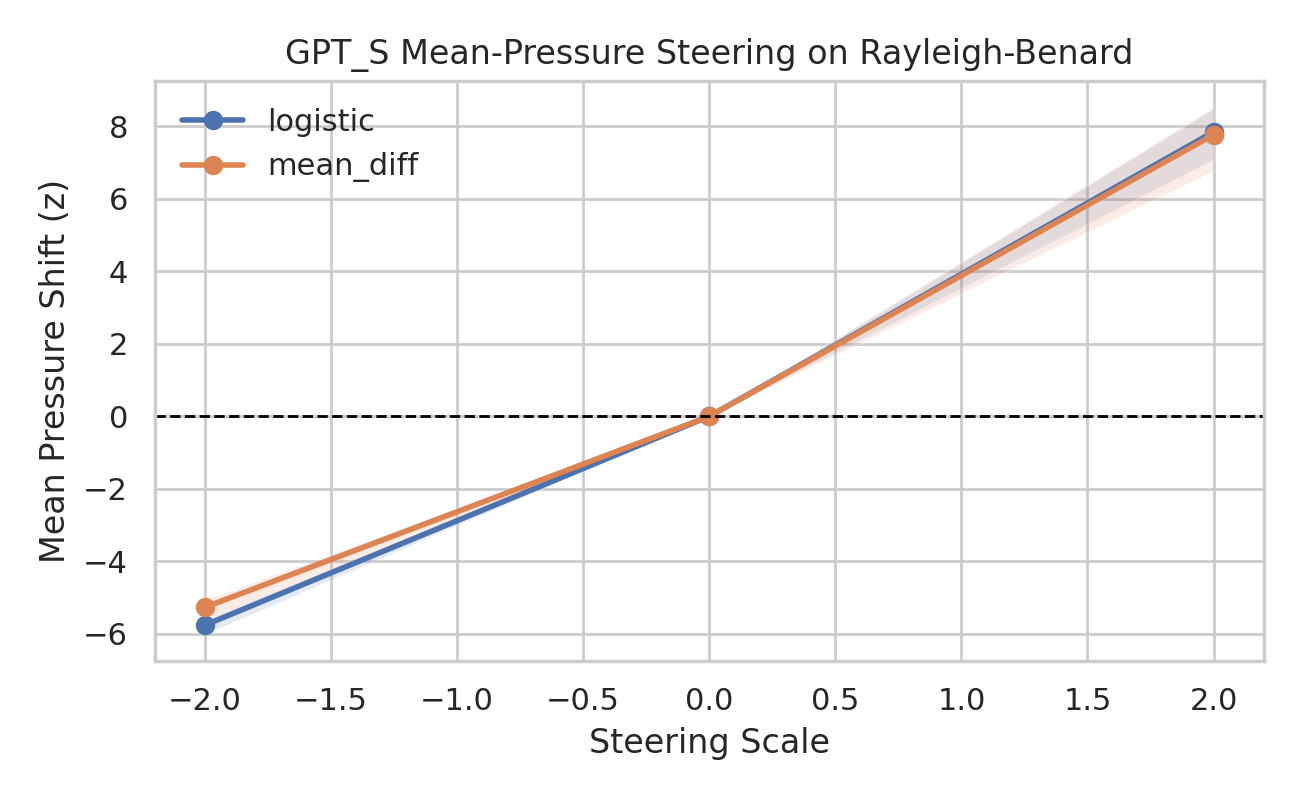
\includegraphics[width=0.8\linewidth]{generated/bootstrap_gpt_s_mean_pressure.png}
    \caption{Pressure steering on GPT\_S. Both fitted directions produce a
    monotonic control signal over the tested scale range.}
\end{figure}

\begin{table}[t]
    \centering
    \caption{Bootstrap steering results for the public GPT\_S checkpoint on
    Rayleigh-Benard validation data.}
    \begin{tabular}{lrlll}
\toprule
Method & Scale & Target Shift & Off-Target Drift & Next-Step MSE Delta \\
\midrule
mean\_diff & -2.000000 & -5.265 & 8.043 & 0.000769 \\
mean\_diff & 0.000000 & -0.000 & 0.000 & -0.000000 \\
mean\_diff & 2.000000 & 7.764 & 1.313 & 0.000498 \\
logistic & -2.000000 & -5.756 & 7.895 & 0.000771 \\
logistic & 0.000000 & 0.000 & 0.000 & 0.000000 \\
logistic & 2.000000 & 7.841 & 1.292 & 0.000530 \\
\bottomrule
\end{tabular}

\end{table}

\section{Interpretation}

The bootstrap report already shows strong directional control: negative scales
decrease predicted mean pressure, positive scales increase it, and the no-op
scale remains numerically stable. The steering effect is large compared with the
baseline variation, while next-step MSE deltas remain on the order of
\(10^{-4}\) to \(10^{-3}\) for the tested scales.

\section{Next Steps}

The remaining work is to broaden the current bootstrap into the full study:
\begin{itemize}
\item repeat the pipeline across GPT\_M, GPT\_L, and GPT\_XL,
\item extend the task set to regime steering and derived-physics features,
\item add steered long-horizon rollout metrics,
\item complete transfer experiments on held-out public datasets, and
\item replace this working draft with the full paper.
\end{itemize}

\end{document}
